\documentclass[../main.tex]{subfiles}
\begin{document}

Bayes 学派看待世界的视角与频率学派不同。简单来说,在 Bayes 方法中,对未知参数 $\theta$ 的认知可以由概率分布来刻画,设对应的随机变量为 $\Theta$,则 $\theta$ 为 $\Theta$ 的实现值。在搜集数据前对 $\Theta$ 的分布的认知 $f_\Theta(\theta)$ 称为\emph{先验分布}。将试验观测抽象为随机变量 $X$,当参数为 $\theta$ 时,观测数据的分布为 $f_{X|\Theta}(x|\theta)$,称为\emph{样本分布}。当观测到数据 $x$ 后,可以利用 Bayes 公式来更新对 $\Theta$ 的认知,得到\emph{后验分布} $f_{\Theta|X}(\theta|x)=\frac{f_{X|\Theta}(x|\theta)f_\Theta(\theta)}{f_X(x)}$。这样,我们就可以利用后验分布来对 $\Theta$ 进行推断。

\begin{example}
    某枚硬币正面向上的概率为未知参数 $\theta$,设先验分布为 $f_\Theta(\theta)=1\ (\theta\in(0,1))$(无信息先验,体现了所谓的同等无知原则,是 Bayes 统计常用假设)。现抛硬币 $n$ 次,观测到正面向上的次数为 $x$。\\
    记 $X$ 为 $n$ 次中正面向上的次数,则给定 $\theta$ 时,$X\sim B(n,\theta)$,即样本分布 $f_{X|\Theta}(x|\theta)=\tbinom nx\theta^x(1-\theta)^{n-x}\ (x=1,\cdots,n)$。于是 $X$ 与 $\Theta$ 的联合分布为 $f(x,\theta)=f_{X|\Theta}(x|\theta)f_\Theta(\theta)=\tbinom nx\theta^x(1-\theta)^{n-x}$,$X$ 的边缘 PMF 为 $f_X(x)=\int_0^1f(x,\theta)\mathrm d\theta=\tbinom nx\int_0^1\theta^x(1-\theta)^{n-x}\mathrm d\theta=\tbinom nx\frac{\Gamma(x+1)\Gamma(n-x+1)}{\Gamma(n+2)}=\frac1{n+1}$,则后验分布为 $f_{\Theta|X}(\theta|x)=\frac{f_{X|\Theta}(x|\theta)f_\Theta(\theta)}{f_X(x)}=\frac{\Gamma(n+2)}{\Gamma(x+1)\Gamma(n-x+1)}\theta^x(1-\theta)^{n-x}$,即 $\Theta|X=x\sim\beta(x+1,n-x+1)$。
\end{example}

其中,$\Gamma(x)=\int_0^{+\infty} t^{x-1}e^{-t}\mathrm dt$ 为 Gamma 函数,满足 $\Gamma(x+1)=x\Gamma(x)$,$\Gamma(1)=1$,对于正整数 $n$,$\Gamma(n+1)=n!$。而 $\beta(a,b)$ 表示 \emph{Beta 分布},其 PDF 为 $f(x)=\frac{\Gamma(a+b)}{\Gamma(a)\Gamma(b)}x^{a-1}(1-x)^{b-1}\ (x\in(0,1))$。若 $X\sim\beta(a,b)$,则 $\mathrm E(X)=\frac a{a+b}$,$\mathrm{Var}(X)=\frac{ab}{(a+b)^2(a+b+1)}$。均匀分布 $U(0,1)$ 即 $\beta(1,1)$ 分布。

上例中,若 $n=20,x=13$,则后验分布为 $\beta(14,8)$,其 PDF 图象如~\ref{fig:6.5.1}。计算可知,$P(\Theta>\frac12)\approx0.91$,而 $\Theta<\frac14$ 的可能性很小。

\begin{figure}[!h]
    \centering
    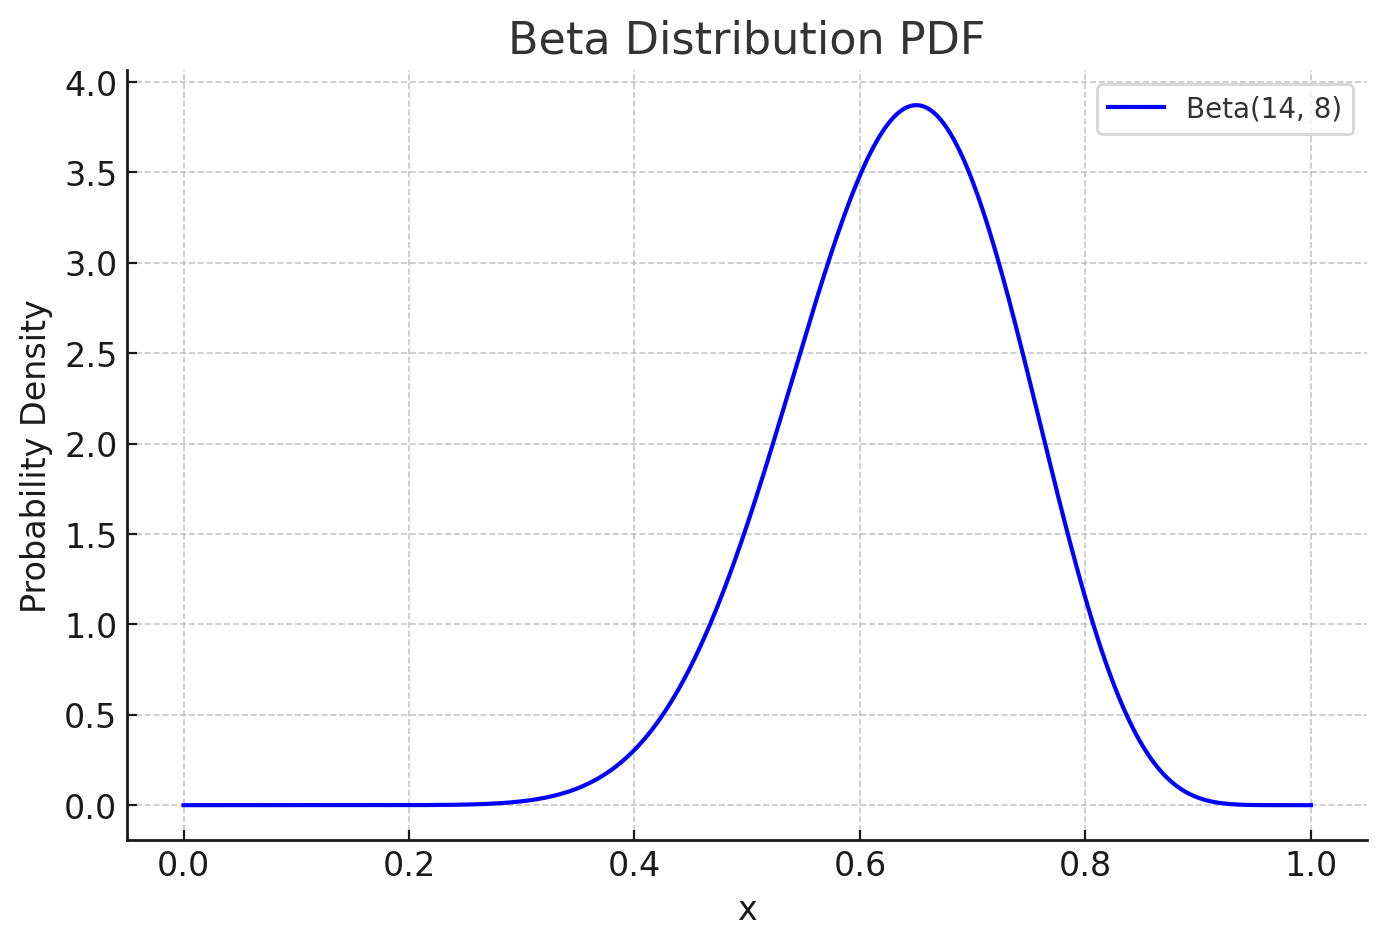
\includegraphics[scale=0.4]{figures/beta(14,8).png}
    \caption{$\beta(14,8)$ 的 PDF 图象}
    \label{fig:6.5.1}
\end{figure}

已知了后验分布后,如何给出参数 $\theta$ 的合理估计呢?常用方法如:
\begin{enumerate}
    \item 后验众数 $\hat\theta_1$,即 $\beta(x+1,n-x+1)$ 的 PDF 最大值点 $\frac xn$(恰与 MLE 一致)
    \item 后验均值 $\hat\theta_2=\mathrm E(\Theta|X=x)=\frac{x+1}{n+2}$
    \item 后验中位数 $\hat\theta_3$
\end{enumerate}

上例中还可以进一步证明,若选取先验为 $\beta(a,b)$,则后验分布为 $\beta(x+a,n-x+b)$,此时后验均值为 $\frac{x+a}{n+a+b}=\frac{a+b}{n+a+b}\frac{a}{a+b}+\frac{n}{n+a+b}\frac{x}{n}$,即后验均值是先验均值 $\frac a{a+b}$ 与样本均值 $\frac xn$ 的加权平均,权重分别为 $\frac{a+b}{n+a+b}$ 和 $\frac{n}{n+a+b}$。

Bayes 方法根据后验分布给出区间估计,称之为 \emph{可信区间}。具体来说,就是要找到 $a,b\in\mathbb R$,使 $P(a<\Theta<b|X=x)\geq1-\alpha$。具体的选取方式如:
\begin{enumerate}
    \item 最大后验区间(通常用于单峰情形),可以直观理解为用一条平行于横轴的线自上而下扫描,直到截取后验 PDF 的面积为 $(1-\alpha)$
    \item 等尾区间,即令 $P(\Theta<a|X=x)=P(\Theta>b|X=x)=\frac\alpha2$
\end{enumerate}

\begin{example}
    设总体分布为 $X\sim N(\mu,\sigma^2)$,其中 $\sigma^2$ 已知,有随机样本 $X_1,\cdots,X_n$,取 $\mu$ 的先验分布 $f(\mu)\propto 1$(无信息先验,这不是一个合理的分布,理解为一种广义 PDF),则样本分布为 $f(x_1,\cdots,x_n|\mu)\propto\prod_{i=1}^ne^{-\frac{(x_i-\mu)^2}{2\sigma^2}}$,后验分布为 $f(\mu|x_1,\cdots,x_n)\propto f(x_1,\cdots,x_n|\mu)f(\mu)\propto\prod_{i=1}^ne^{-\frac{(x_i-\mu)^2}{2\sigma^2}}\propto e^{-\frac{n\mu^2-2\mu\sum_{i=1}^nx_i}{2\sigma^2}}\propto e^{-\frac{n(\mu-\bar x)^2}{2\sigma^2}}$,即 $\mu$ 的后验分布为 $N(\bar x,\frac{\sigma^2}{n})$。
\end{example}

\end{document}
